\documentclass[manuscript]{aastex}
\newcommand{\vdag}{(v)^\dagger}
\newcommand{\ie}{{\it i.e., }}
\newcommand{\eg}{{\it e.g., }}
\newcommand{\myemail}{steinkirch@gmail.com}



\begin{document}


\title{On the Spectroscopy Study of the Earthshine Spectra}
\author{{\bf Marina von Steinkirch} \\ (laboratory partners: A. Massari and M. von Hippel)}
\affil{State University of New York at Stony Brook \\ Department of  Physics and Astronomy  }
\received{: \today}
\accepted{: \today}



\begin{abstract}
We obtain a low-resolution optical spectrum of the faint glow from the dark side
of the Moon, \ie the Earthshine.  We extract  the 
Earth's spectrum from it and observe absorption features of ozone, molecular oxygen, and
water. The  spectra is fitted to five
well-known models for the atmosphere and the ground of a planet with life
content. At short wavelengths, the largest
contribution to this spectra comes from Rayleigh scattering. At long
wavelengths, enhancements  with values of $4\pm 5\%$ starting at 740 nm were
found, corresponding to the red
reflectivity edge of vegetation. 

\end{abstract}
\keywords{Earthshine $\cdot$ Earth's Spectrum $\cdot$ biosignature}






\section{Introduction}
% a contextual description of the goals of experiment


The detection of {\it exolife} is one of the most important goals for
future space missions. Current space missions used to identify exoplanets
include \texttt{COROT}, \texttt{Spitzer} and \texttt{the Hubble Space
Telescope}, as well as the secondary extended mission of \texttt{Deep Impact
(EPOCh)} which will observe the light reflected from exoplanets
\cite{arnold_etal07}. \texttt{ESA’s Darwin} mission (estimated launch 2015)
will aim to find and study the properties and composition of Earth-like
exoplanets in the infrared. Over 300 giant exoplanets already have been
detected, and hundreds, perhaps thousands more, are anticipated in the coming
years. The nature of these planets, including their orbits, masses, sizes,
constituents, and likelihood that life could develop on them, can be probed by a
combination of observations and modeling.

Our observations tie in with current and future missions to observe and
search for life on exoplanets. By looking at the spectra of Earth, we can
characterize what makes it suitable for sustaining life - information that can
be related to present and future exoplanet observations. This search is
characterized by the detection of possible {\it biomarkers} on Earth-like
exoplanets. On a first approach, they are simple molecules present in the
planet's atmosphere, such as $O_2, O_3, CO_2,$ and $H_2O$ (see Fig.\ref{1}-a).
Further studies aim for the detectibility of a proper signature of life from
the planet's surface, considering, for instance, green vegetation as a biormaker
\citep{seager_etal05}.


Solar's photon flux reaches the ground after absorption through Earth's
atmosphere. In this case, vegetation reflects or transmits almost all
incident radiation at
wavelengths where sunlight has about 40$\%$ of its energy. The {\it vegetation
reflectance} (vegetation spectral signature) has a well know
spectrum, with a sharp edge of $\lambda =  700$ nm in the visible
electromagnetic spectra due to the missing photons used in photosynthetic
process. This is detected as a {\it positive shift} above the continuous
spectra, starting at
this wavelength, also known as the {\it Vegetation Red Edge} (VRE) (see
Fig. \ref{1}-b).


\begin{figure}[h]
\begin{center}
 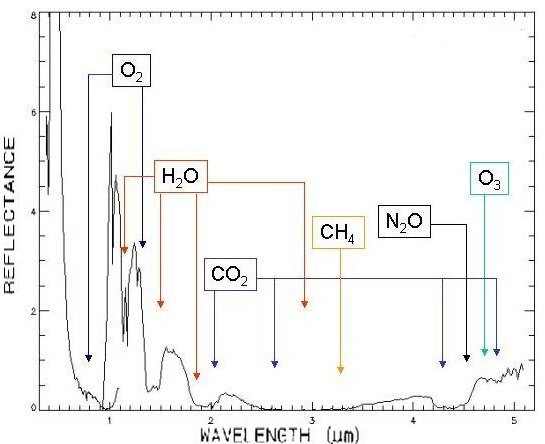
\includegraphics[width=0.45\textwidth]{figs/1.jpg}
 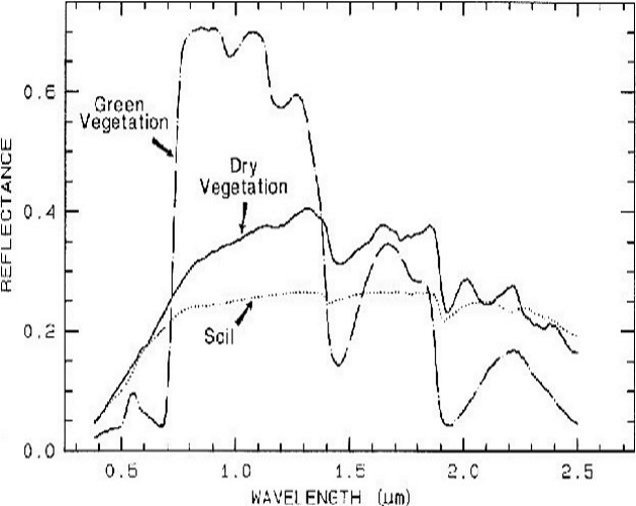
\includegraphics[width=0.45\textwidth]{figs/2.jpg}
\caption{\footnotesize (i) Mars Express record of Earth
spectrum on the visible, (ii) The vegetation spectral signature.}
\label{1}
\end{center}
\end{figure}





\subsubsection*{The Earthshine as a Tool to the Study of other Earth-like
Systems}

The observation of the spectrum of {\it Moon Earthshine}, \ie the reflection of
the Earth's light on the non-sunlit Moon, allows one to observe the
Earth as any distant planet, and to perform studies on the detectibility of
biomarkers ({\it e.g.} VRE) in its spectrum. Extracting the Earth albedo from
the Earthshine spectrum requires the measurement of moonlight spectra (lit side
of the moon) and the Earthshine spectra (unlit portion of the moon) in the
visible wavelength \citep{woolf_etal02} (see Fig. \ref{2}).



\begin{figure}[h]
\centering
 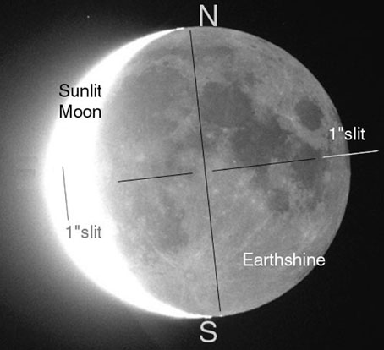
\includegraphics[scale=0.45]{figs/4.png}
 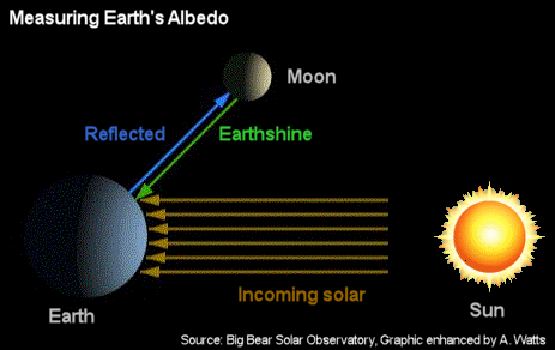
\includegraphics[scale=0.45]{figs/3.png}
\caption{\footnotesize (i) Moon's Earthshine and the schematic illustration of
the dark and bright side of the moon, (ii) Schematic illustration of the
sunlight reflected from the the Earth.}
\label{2}
\end{figure}


The spectrum of the light reflected by the planet, when normalized to the Sun
(parent star spectrum), gives the planet reflectance spectrum revealing its
atmospheric and ground color (if this is visible by a transparent
atmosphere). Quantitatively, the Earth spectrum from the Earthshine depends on
the following
variables:
\begin{itemize}
 \item the Sun spectrum as seen from outside of Earth's atmosphere, $S(\lambda)$,
\item  the Earth's atmospheric transmittance, $AT(\lambda)$,
\item the moonlight (sunlight reflected by the Moon's surface), $MS(\lambda)$,
\item the earthshine, $ES(\lambda)$,
\item the lunar reflectance, $MS(\lambda)$,
\item the Earth's reflectance, $ER(\lambda)$.
\end{itemize}

So we can write
$$ MS(\lambda) = S(\lambda) \times MR(\lambda) \times AT(\lambda) \times g_1,$$
and
$$ ES(\lambda) = S(\lambda) \times ER(\lambda) \times MR(\lambda) \times
AT(\lambda) \times g_2.$$

The Earth's reflectance is given by the ratio of the two equations,
\begin{equation}
 ER(\lambda) = \frac{ES(\lambda) g_1}{MS(\lambda) g_2},
\label{skyy}
\end{equation}
where $EM(\lambda)$ and $MS(\lambda)$ should be recorded simultaneously to avoid
airmass variation, and $g_1, g_2$ are geometric factors related to the position
of Sun, Moon and Earth, and they can be set to unity. 


The {\it vegetation red edge} is extracted from $ER(\lambda)$,
\begin{equation}
 VRE = \frac{r_I-r_R}{r_R},
\label{vge}
\end{equation}
where $r_I$ and $r_R$ are the near  infrared and red reflectance integrated over
the spectral domains ($\sim$ 10 nm width) \cite{arnold_etal07}
\cite{arnold_etal02} \cite{writeup}.



\section{Observations}

This experiment aims to obtain an optical spectrum of Earthshine and test for
the presence of biomarker features,\eg O$_2$, O$_3$, H$_2$O, and the presence of
the vegetation red edge through fits of several models' components to the
observed spectrum. The observations were performed on the {\bf Mt. Stony Brook
14-inch telescope}, with the {\bf DADOS optical spectrograph} \cite{dados}, and
the {\bf SBIG STL-402 CCD camera} \cite{CCD}, on the date of April 17th, from
1:30 am to 5:30 am. The sky was clean and the temperature was around
55$^{\circ}$ F. The overall cloud cover from the archival satellite imagery and
the Earth seen from the moon, can be seen in the figures \ref{sat} and
\ref{frommoon},  in the appendix.




\subsection{Setting up the Spectrometer}
A spectrometer  splits the incoming light
of Earthshine by wavelength, having previously been focused by the optical
section of the instrument. The intensity of light at each wavelength is
measured and recorded by the detector, and it is then  plotted  against light
intensity, which is analyzed to find a number of
features. In order to pick up the key features of oxygen, water and vegetation
red edge, we investigate the visible and near infrared sections of
the electromagnetic spectrum, with light of wavelengths between  500 to
800 nm.






Earthshine is brightest when most of the Earth as seen from the Moon is
illuminated, {\it i.e.}, when the Moon is only a thin crescent. However, if the
Moon is too close to the Sun, there are  difficulties  separating
the glow of Earthshine from the bright twilight sky \cite{woolf_etal02}.
We select  a  night of waxing crescent moon when  the angular separation from
the Sun to the moon (from the moonrise to the sunrise) is suitable for the
experiment. This means that   the moon is sufficiently high above the
horizon ($>20^{\circ}$), yet sufficiently close to the Sun
($<90^{\circ}$) so that the Earthshine signal is bright.  The observations
cease at sunrise, since when the Sun reaches about 5$^{\circ}$ below the
horizon, the sky will  be too bright  to measure Earthshine. 



We set the optical wavelength range of the spectrograph to cover our chosen set
of Earthshine absorption by molecular O$_2$, O$_3$, H$_2$O. This was done before
mounting the spectrograph on the telescope with the help of the Neon light
source. We looked up the  wavelengths of the strongest Neon gas transitions
in the optical, adjusting the wavelength range of the spectrograph. We use the
DADOS spectrograph with long integration times. To maximize the spectral
resolution the narrowest width slit $ 25 \mu m$ is to be used. This gives a
spectral resolution of $\lambda / \Delta \lambda \sim 500$.


Setting  the telescope tracking rate to lunar ({\texttt Autostar II}
keypad), we obtain sequences of spectra of the {\bf bright} (moonshine) and {\bf dark} (earthshine) sides
of the facing Moon, each of them together with  the adjacent {\bf sky} (in the
adjacent slit). We also take
calibration exposures of the Neon light source and  darks with duration matched
to the duration of all of the science exposures.

\subsection{Estimative of Exposure Times}

The Earthshine  usually has low S/N (signal to background) ratio because the
observations are obtained with Moon low above the horizon, and consequently a
high airmass and low Earthshine fluxes with respect to the sky. Moreover, the
detector can be quickly saturated when recording the spectrum of the sunlit Moon
crescent. When it comes to the vegetation signal, the Earthshine data reduction
becomes even more difficult: past works \cite{seager_etal05} have
shown that it  is only a few percent (less than $5\%$) above
the continuum. Two reasons for this are pointed in the literature: (i) the variable amplitude, induced by a variable cloud cover and the Earth phase, (ii) the strong astmospheric bands which need to be removed to access the surface reflectance. 

Assuming that the signal is limited to photons, the signal to background ratio
for each of the sciences can be written as
\begin{equation}
 S/N = \sqrt{N_{\gamma}t},
\end{equation}
where $t$ is the time of integration ans $N_{\gamma}$ the number of photon
counts.

First, we make an estimate of the exposure time for the dark and
the bright side of the waxing crescent moon, supposing that their S/N are
similar. Considering that the {\it full moon} has magnitude
$m_{full} = -12.7$ and the {\it new moon} has magnitude $m_{new}= -2.5$, the
ratio of {\it photon fluxes} for the dark and bright side of the moon \cite{CCD}
is
\begin{eqnarray}
 R_{d/b} &\sim&\frac{F_{dark}}{F_{bright}}, \nonumber \\ 
&\sim& 0.1 \times 10^{(m_{full} - m_{new}) / 2.5}, \nonumber \\
&\sim& 10^{3}. \nonumber 
\end{eqnarray}

We can then derive the exposures times for each side,
\begin{eqnarray}
 t_{bright} \times N_{\gamma \, bright} &\sim& t_{dark} \times N_{\gamma \,
dark} \times R^{-1}_{d/b}.
\nonumber
\end{eqnarray}

The last result means that if we keep the number of counts constant for the dark
and bright sides, we should aim for calibration dark exposure times of
around 1000 
larger than those for bright, \eg we should have at least 90 minutes of net
observation of the dark side for a 5 seconds exposure of the bright side.
However, due the observational constrains, we ended up collecting only 1/4 of
this value, as it is shown in the Table \ref{looo} of the
appendix.




\subsection{Steps of Data Acquisition}

The data acquisition was  performed by the following steps, based on the
exposure times in the Table \ref{looo} in the appendix:
\begin{enumerate}
\item We record the spectrum of the Neon lamp on all the slits.

 \item We record a non-saturated spectrum of a {\it  bright stellar point
source} (Altair) at {\it two distinct positions on the slit}. We trace their
spectrum, which gives the direction along which we extract the spectrum of  the
Earthshine.

\item We track the {\it dark side of the Moon},  positioning the {\it dark limb}
in one slit and the adjacent on the other and recording the spectra.

\item We measure  the {\it illuminated limb of the moon } in the same way,
with a much smaller time to avoid saturation.

\item We repeat the above three procedures while the Sun is still not close
enough to the Moon.
\item   We obtain sets of dark frames for all the  exposure times of
our sciences.
\end{enumerate}











\section{Data Reduction}
% description of how reduced and calibrated  your data

The CCD observations are registered as astronomical images (FITS, Flexibble
Image Transport System). All the
analysis was done in IDL and ATV \cite{atv} - the source codes are
included in the appendix.




\subsection{CCD Dark Frame Calibration}

The first step of the data reduction is to remove the various instrumental
artifacts of the CCD, by calibrating  the science images. We create {\it dark
master frames} for every exposure times, \ie median combined frames of the CCD
closed, the high signal-to-noise dark. We subtract these frames from the
respective science frames with same exposure times and median combine these
last to form a deep exposure frame.


\subsection{Spectra Trace Calibration}

Spectra are arranged on the CCD in a manner that most efficiently makes
use of the detector size/area. Before these spectra can be extracted, their
exact positions on the CCD must be mapped. This is the process of {\it 
aperture tracing}. To this, we calculated the  spectra's {\it trace} from two
methods:
\begin{enumerate}
 \item Method 1: From a standard point source;
\item Method 2: By integrating the 1 + 1/2 strips.
\end{enumerate}

The trace of the point source, \eg a bright
(standard) star in the sky, is taken by positioning this star in each of the
three slits.
With ATV \cite{atv}, it is possible to extract the {\it spectral flux
distribution} \footnote{Loading the image with \texttt{decomposed, device=0}
option and pressing \texttt{x} on it.}, $F_{\lambda}$,  as shown in the Fig.
\ref{f}.

\begin{figure}[htb]
\begin{center}
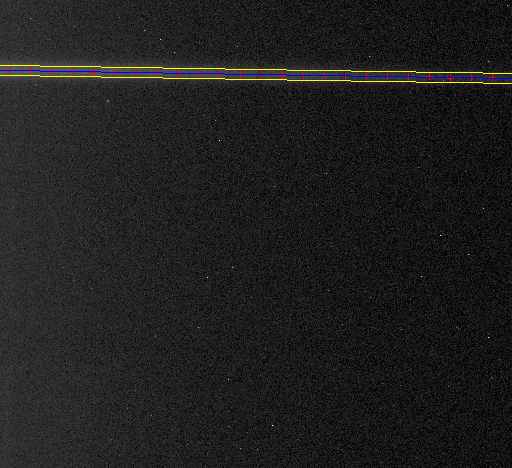
\includegraphics[scale=0.25]{plots/trace/point2.png}
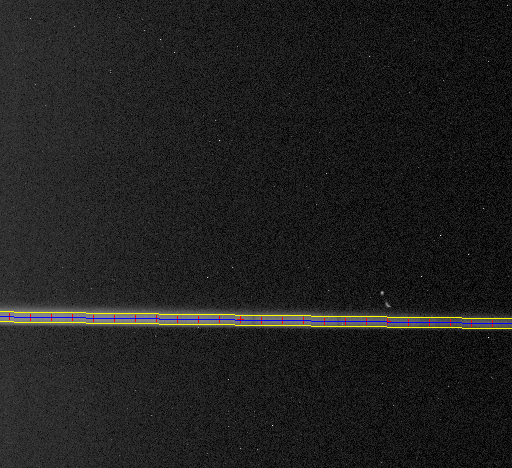
\includegraphics[scale=0.25]{plots/trace/point3.png}
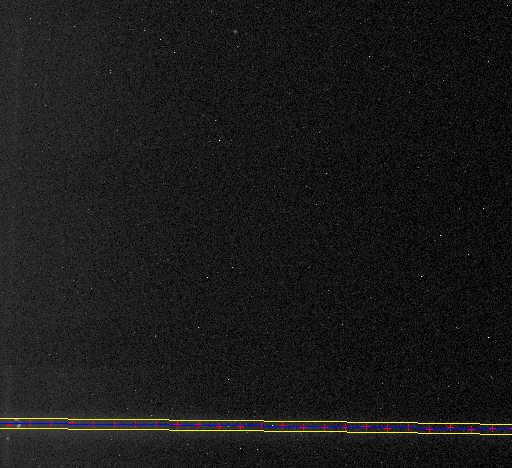
\includegraphics[scale=0.25]{plots/trace/point1.png}
\caption{Trace extraction from a point source  star in each of the three
slits
(from ATV).}
\label{f}
\end{center}
\end{figure}

 For the Moonshine, the flux is very high and using only the the point
source trace (method 1) was enough.
(see Figs. \ref{star-cal}).



\begin{figure}[htb]
\begin{center}
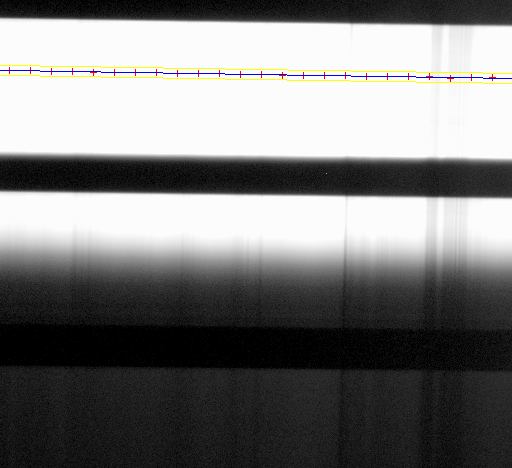
\includegraphics[scale=0.33]{plots/trace/moon.png}
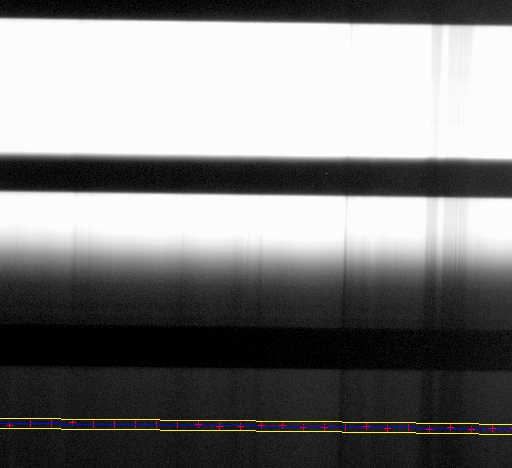
\includegraphics[scale=0.33]{plots/trace/moonsky.png}
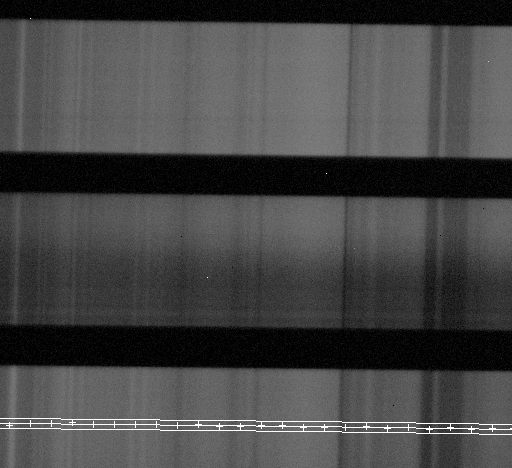
\includegraphics[scale=0.33]{plots/trace/earth.png}
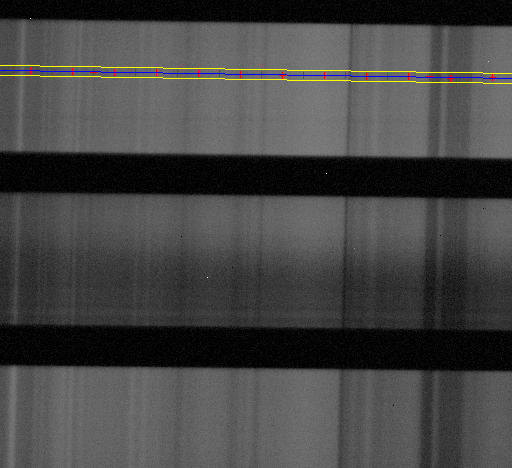
\includegraphics[scale=0.33]{plots/trace/earthsky.png}
\caption{Extraction of the point source spectra for the bright (above) and dark
(below) side of the
waning crescent moon and its adjacent sky (from ATV).}
\label{star-cal}
\end{center}
\end{figure}


Only for the Earthshine, due
to their much lower signal (in the same order of the adjacent sky), we determine
a second set of data (method 2), aiming to extract more statistics from the
data. We proceeded integrating over the whole
Earthshine strip and adding half of the middle strip (which has the adjacent
sky on the other half).





\subsection{Adjacent Sky Subtraction}
Both the dark and bright side of the Moon are corrected for scattered
light in the telescope by subtracting the adjacent sky spectrum. The adjacent
skies were always extracted in the same way the their respective set of data. The
sky-subtracted spectra can been in the see Figs. \ref{comparing}. 



\begin{figure}[htb]
\begin{center}
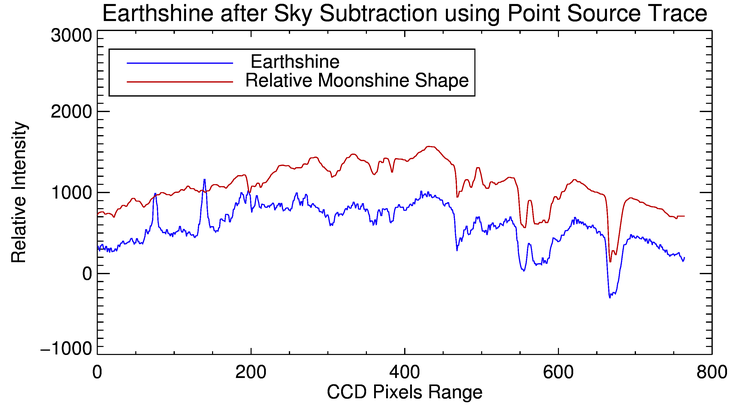
\includegraphics[scale=0.31]{plots/earth_point.png}
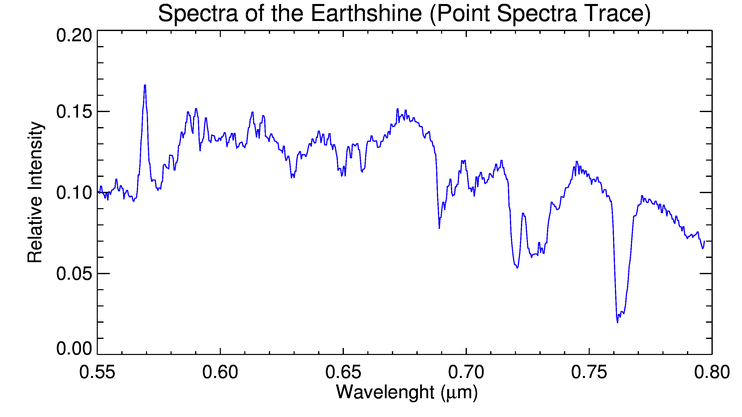
\includegraphics[scale=0.31]{plots/spectra1.png}
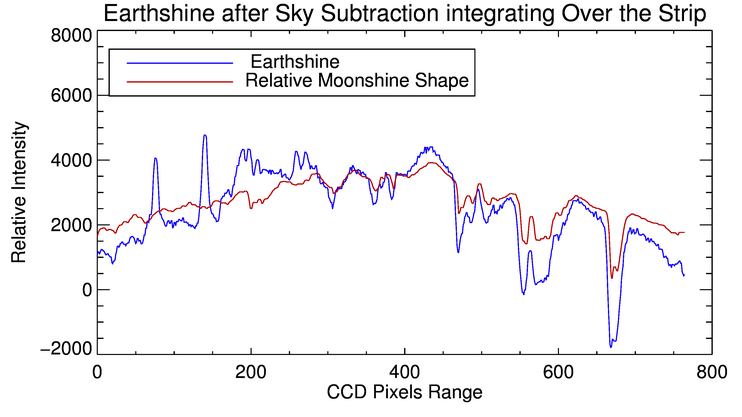
\includegraphics[scale=0.31]{plots/earth_strip.png}
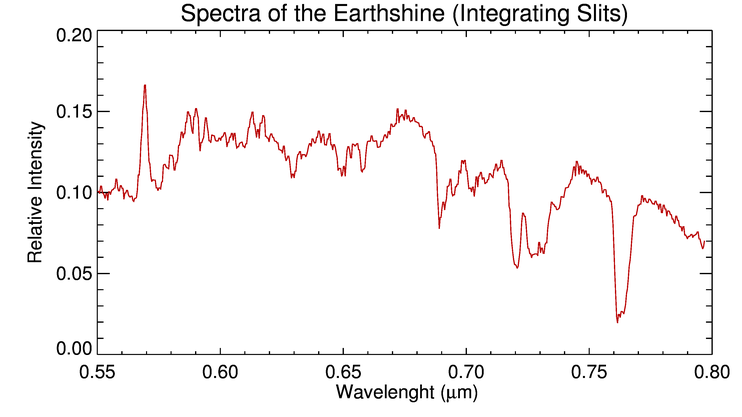
\includegraphics[scale=0.31]{plots/spectra2.png}
\caption{Earthshine spectra from method 1(top) and method 2 (down), comparing
to the scaled Moonshine spectra, in function of CCD pixel counts, and
wavelength calibrated.}
\label{comparing}
\end{center}
\end{figure}

After these
reductions we were able to calculate the signal
to background for
the Earthshine (methods 1 and 2) and for the Moonshine spectra, obtaining
$S/N^{point}_{earth} = 1.8$,  $S/N^{strip}_{earth} = 3.4$ and
$S/N_{moon} = 148$, respectively.

\subsection{Obtaining the Reflectivity of Earth}


The reflectivity of Earth is the ratio of the Earthshine to the Moonlight
spectra, \ie by reducing the contribution of the extra
passage of the Sun through the Earth's atmosphere in the spectrum of the
Earthshine. Dividing  the dark side by the bright side (the earthshine by the
 moonshine) for methods 1 and 2, we obtain the Fig. \ref{comparing2}. We
confirm that they show a very good agreement, with  a very small enhancement
from the method 2. We shall use only this spectra on the following analysis and
refer to it as the Earthshine reflectivity. 


\begin{figure}[htb]
\begin{center}
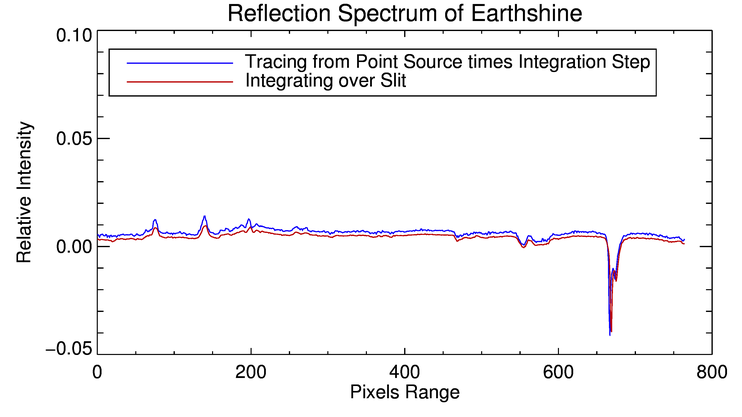
\includegraphics[scale=0.6]{plots/reflectivity0.png}
\caption{Earthshine reflectivity from method 1 and 2, scaled to each
other.}
\label{comparing2}
\end{center}
\end{figure}








\subsection{Absolute Spectra Calibration}
To obtain the absolute wavelengths of the Earthshine spectrum, we measure the
spectrum of a neon calibration lamp and compare it to the well-known wavelengths
of neon
transitions, see Fig. \ref{fig-neon}.

\begin{figure}[htb]
\begin{center}
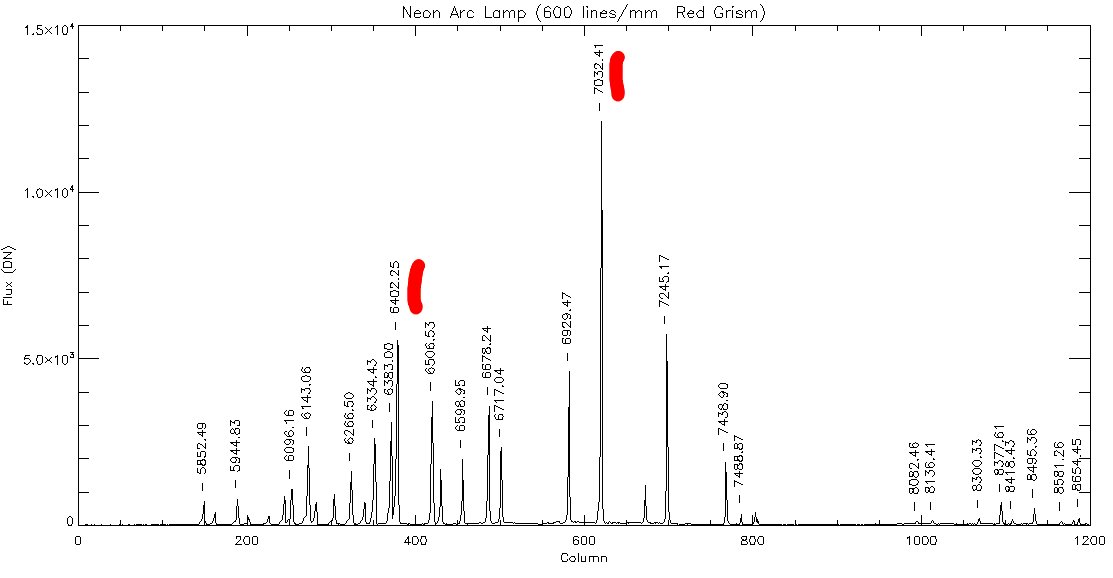
\includegraphics[scale=0.2]{figs/neon.jpg}
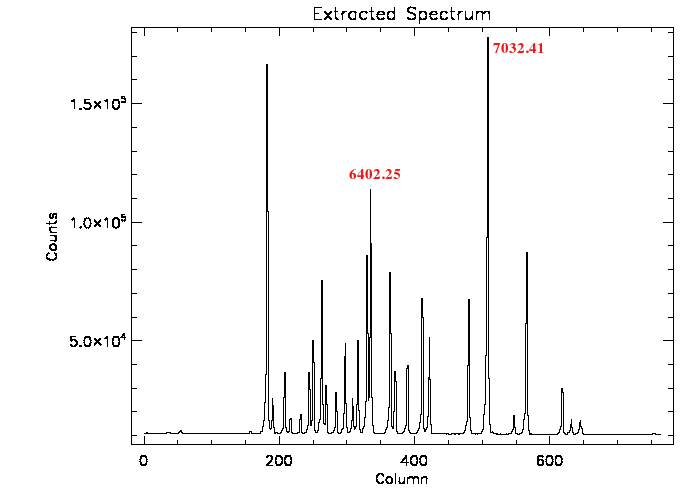
\includegraphics[scale=0.45]{plots/neon1.png}
\caption{Wavelength transitions of neon: (left) from the literature
\cite{neon-wave}, (right)  experimentally obtained.}
\label{fig-neon}
\end{center}
\end{figure}

We find the {\it $\lambda$/pixels scale dispersion} and we reduce the
Earthshine spectra from it.This results on the Earthshine spectra 
correlation to light wavelengths, \ie the reflectivity of the Earth.

\begin{figure}[htb]
\begin{center}
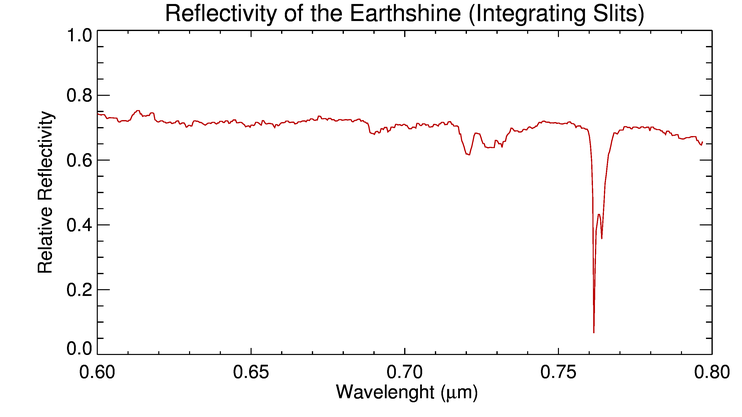
\includegraphics[scale=0.6]{plots/reflectivity2.png}
\caption{The Reflectivity of the Earth.}
\label{fig-es}
\end{center}
\end{figure}






\section{Data Analysis and Results}
% description of any analytically steps: parameter estimation, error estimation, model-fitting...

\subsection{Detecting Molecular Gas Features}

We compare the final sky-subtracted and wavelength calibrated spectrum of the
Earthshine to predictions and existing measurements. First, we
detect the molecular bands of O$_2$, O$_3$, and H$_2$O by comparing the
 absorption lines obtained from \cite{nuclear}.  We verify that the abundance of
those components are compatible to the
literature (see  Fig. \ref{mol}). 

\begin{figure}[htb]
\begin{center}
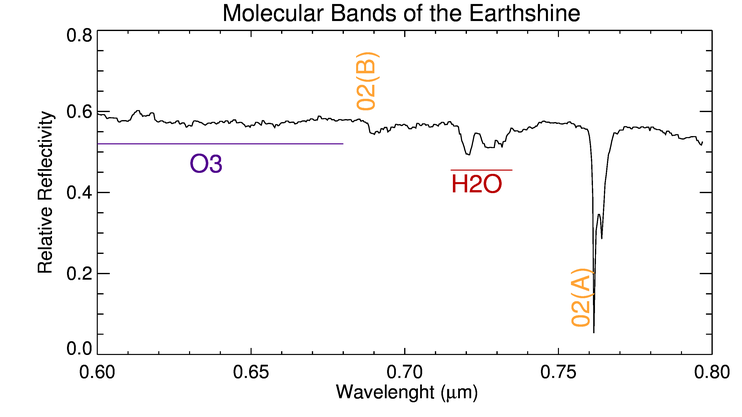
\includegraphics[scale=0.5]{plots/mo1.png}
  \caption{Atmospheric molecular bands detected in the Earthshine spectrum.}
\label{mol}
\end{center}
\end{figure}


The presence of strong
absorption lines in the near infrared when comparing to  shorter regions (blue)
of the spectra indicates that if human vision were sensitive a little further
toward the red, the natural world would be very red and exceeding bright. In the
next session we also see that the blue spectrum from the subsurface ocean water
has a very small contribution ranging for wavelengths around 500 to 600 nm.





\subsection{Detecting the Vegetation Red Edge}

The main contributors to the optical spectrum of Earthshine \cite{writeup}
\cite{USGS} are
\begin{enumerate}
 \item The {\bf neutral reflectivity from high clouds} (same as the Sun
(blackbody) with $T \sim 5700$K and independent of the wavelength).
\item The blue  spectrum of subsurface {\bf ocean water} (see Fig. \ref{veg} (right))
.
\item The {\bf transmission of Earth's  clear atmosphere}.
\item The {\bf Rayleigh scattering} (proportional to $1/\lambda^4$).
\item The {\bf vegetation} reflection spectrum from land chlorophyll
plants (see  Fig. \ref{veg} (left)).
\end{enumerate}



\begin{figure}[htb]
\begin{center}
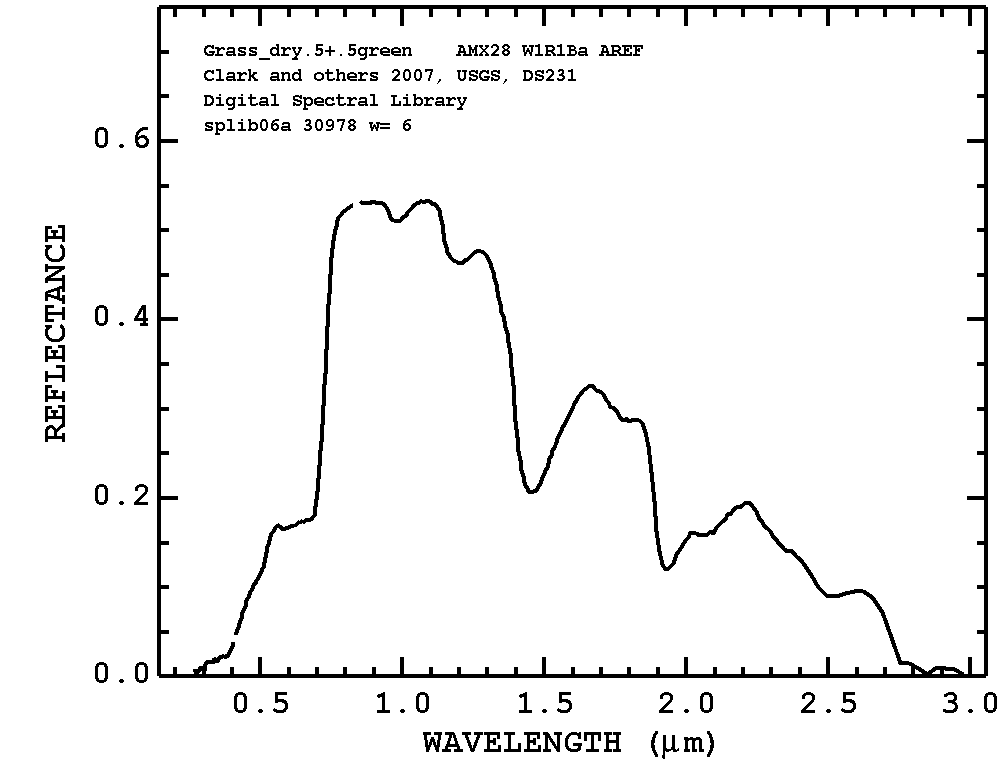
\includegraphics[scale=0.22]{figs/green.png}
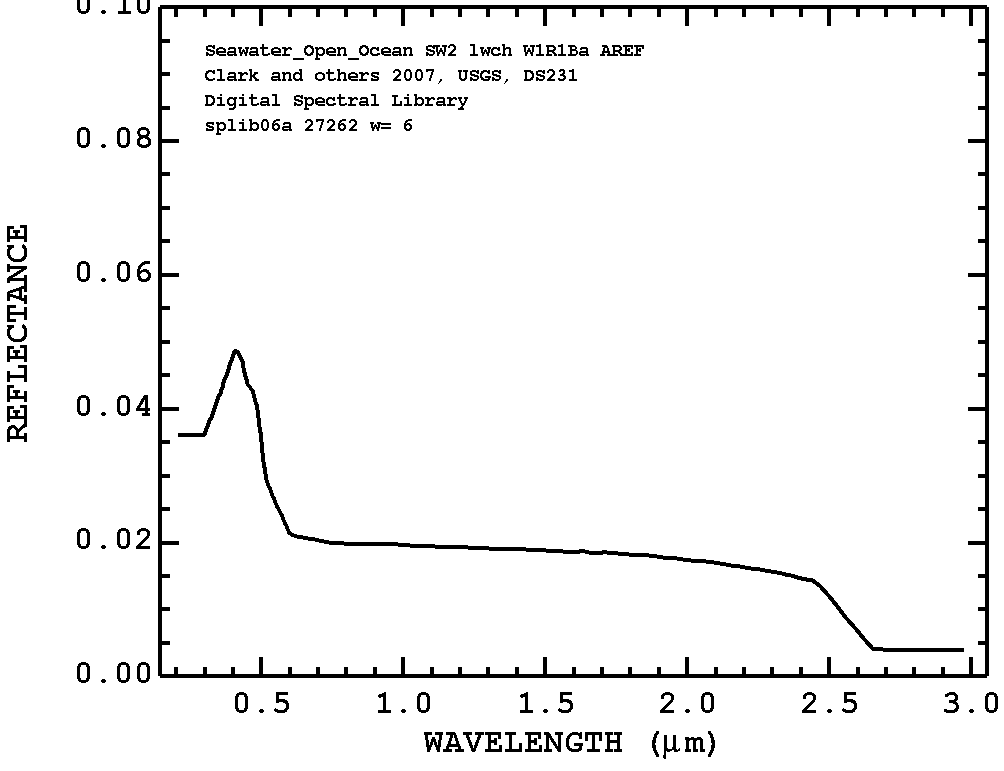
\includegraphics[scale=0.22]{figs/sea.png}
\caption{Some of the models we fitted our spectra: (left) Vegetation reflection
and (right) Ocean Surface.}
\label{veg}
\end{center}
\end{figure}

 We fit together each of the previous five models to our spectra of the
Eartshine, inferring the partial contributions to
the combined spectrum (see Fig. \ref{models}), \ie our model has 5 parameters. We calculate the best values for these parameters
to minimize $\chi^2_{point}$ on each point then integrate to an acceptable
final value of  $\chi^2=7.8$ (see fitting code in ROOT in the appendix). We
assume the data are normally distributed with a variance equal to the mean and
the data points are independent from each other, so we can use the level of
significance of $\alpha >0.1$ for the fit. For five parameters, the $\chi^2_5$
should be less than 9, so we see that our fit is indeed significant: $\chi^2$ is
not too large for a good fit and it is large enough to reject the {\it null
hypothesis} \cite{writeup}.

\begin{figure}[htb]
\begin{center}
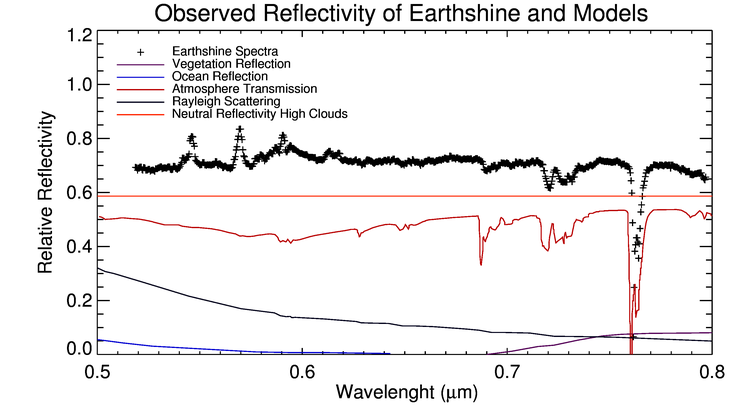
\includegraphics[scale=0.6]{plots/fit.png}
\caption{The main models to the optical spectrum of Earthshine which we fit
to our data. They are scaled in the plot for a better display.}
\label{models}
\end{center}
\end{figure}


The most important components in the fitting are the Rayleigh scattering
(high cloud continuous) in the beginning of the spectra and the clear atmosphere
(molecular spectrum) in the whole range.

We calculate the vegetation edge from equation
\ref{vge}. With mean reflectances in the [600, 670 nm] and [740, 800 nm]
windows in the spectrum, we obtain
$VGE =4 \pm 5\%$, which was small but compatible with
the literature \cite{USGS}.
The errors were estimating by looking at the standard deviation during
a ``flat'' part of the spectra and dividing by the mean in that region. 








%\include{discuss}
\section{Conclusion}
% recapitulation of results and what we learned


The spectrum of the Earth as it would appear to an extrasolar observer is useful
for learning how to analyze the spectra of extrasolar planets. It 
illustrates both atmospheric and surface reflectivity features. 

The main contribuition for the spectra comes from the atmosphere transmission.
We also see enhanced reflectivity at short wavelengths from Rayleigh scattering
and
apparently negligible contributions from aerosol and ocean water scattering.  We
 see enhanced reflectivity of $4\pm 5\%$ at long wavelengths starting at
about
740 nm,
corresponding to the well-known vegetation red-edge. Our fittings for the
Earth's reflection spectrum shows good agreement with the combination of
reflectance, scattering, and transmission models.

The vegetation signal was not very 
significant mostly because of  the difficulties of the observation - we had a
signal-to-background ratios of  S/N $<$ 5. Although the observations
had great part of reflecting land  and had not much high
clouds in the atmosphere (see figures \ref{sat} and \ref{frommoon}), the low
signal is due to the fact that we only had 20 minutes of net observation for the
Earthshine (less than one fourth of the minimum we had estimated in
the beginning of the report).


In conclusion, we have shown that an observer in a nearby stellar
system, with the same or better resources used in this experiment, would be able
to use the oxygen, water and ozone absorption features to suspect the presence
of life on
Earth. The small chlorophyll
red-edge reflection feature might also help to confirm the presence of life.


\input{example_proposal.bbl}
\clearpage


\appendix
\begin{deluxetable}{ccccccccc}
\tabletypesize{\scriptsize}

\tablecaption{DADOS Spectrograph Observations Log Sheet}
\tablewidth{0pt}
\tablehead{
\colhead{File} & \colhead{Object} &\colhead{Exp. Time (s)} & \colhead{Position
in the Slit}  & \colhead{Slit ($\mu
m$)} 
}
\startdata                                                                      
          
 cal/1 & Neon	&1	& in all of them	& 200		\\
cal/2 & Star - Altair	& 30	& middle	& 200		\\
cal/3 & Star - Altair	& 30	& bottom	& 200		\\
cal/4 & Star - Altair	& 60	& top	& 200		\\
bright/15/1-5& Moonshine	& 15
& Sky on top & 200	\\
bright/30/1-5& Moonshine	& 30
& Sky on top & 200	\\
dark/1-10& Earthshine	& 120	& Sky
on bottom & 200	\\
\enddata
\label{looo}
\end{deluxetable}


\begin{figure}[htb]
\begin{center}
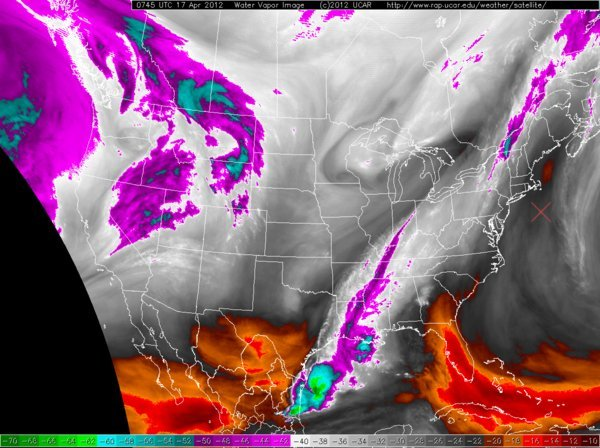
\includegraphics[scale=0.42]{figs/satt.jpg}
\caption{Cloud coverage on Earth for the period of observations.}
\label{sat}
\end{center}
\end{figure}

\begin{figure}[htb]
\begin{center}
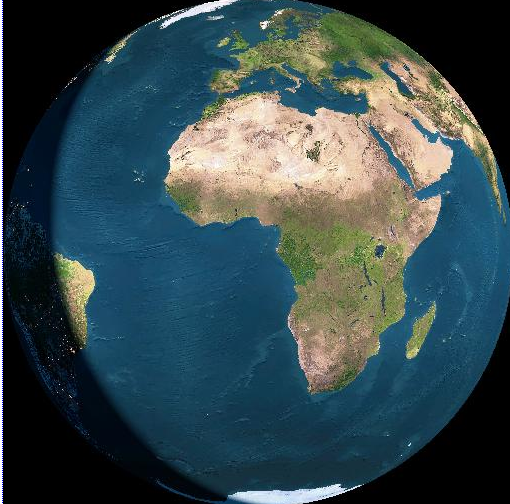
\includegraphics[scale=0.3]{figs/frommoon1.png}
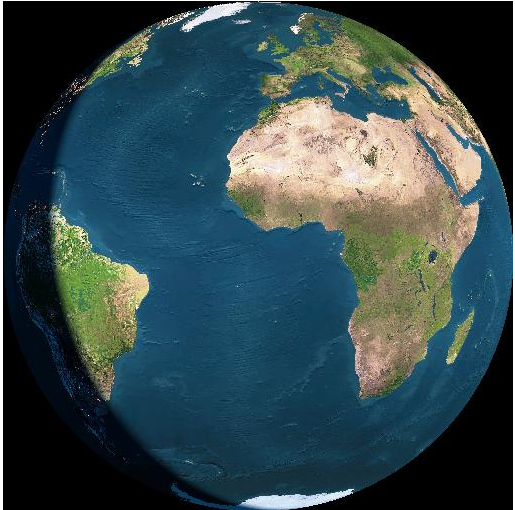
\includegraphics[scale=0.3]{figs/frommoon2.png}
\caption{Earth seen from the Moon in the begin and the end time of our
observations.}
\label{frommoon}
\end{center}
\end{figure}


\begin{figure}[htb]
\begin{center}
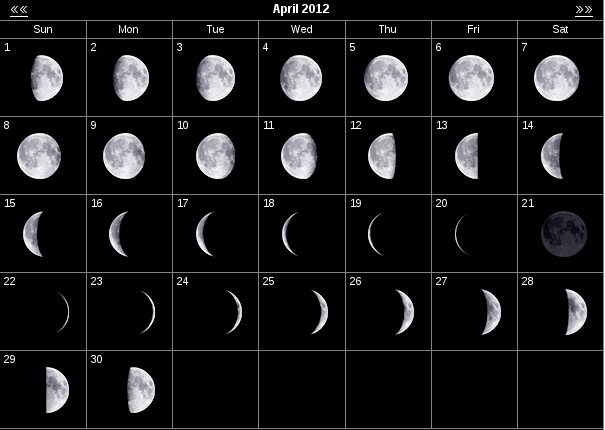
\includegraphics[scale=0.6]{figs/moon.png}
\caption{Phases of the moon for the month we were observing. The data was
taken on the 17th, a waning crescent moon.}
\label{moooon}
\end{center}
\end{figure}





\end{document}
